\SetPicSubDir{ch-Design}
\SetExpSubDir{ch-Design}

\chapter{Design of the system}
\label{ch:design}
\vspace{2em}


\section{Programming Language}

We provide a simple functional language in \autoref{fig:LanAST}. A program
comprises a list of abstract datatype declarations \texttt{datat}, a list of user-defined predicates \texttt{spred} and a list of method declarations
\texttt{meth}. The supscript $*$ is used to denote a list of items. The function
body can be composed by constant $k^{\tau}$ of a ground type $\tau$, a variable $v$, a lambda expression $e$ with a bounded variable $v$, 
function application of two expressions, if branches, pattern matching on datatype
expressions, and primitive operations (such as arithmetic and boolean operations).

Following the OCaml programming convention, a program is presented as a 
list of \texttt{let}\zz{}expressions, each of which declares a method to be
verified. In order to allow users to write specifications, each method
declaration should come with a function specification $\mathcal{F}$. 
We also allow users to provide predicate instances $\texttt{spred}$ in
the program. The syntax of function specification $\mathcal{F}$ and 
logical proposition $\pi$ will be described in the next section.

\begin{figure}[htp]
$$\begin{array}{rrl}
    \text{program}: & \texttt{P} := &\texttt{datat}^* \ \texttt{spred}^* \ \texttt{meth}^* \\
    \text{data type}: & \texttt{datat} := & \texttt{type } \mathbf{c} \texttt{ = } \texttt{tconstr}^* \\
    \text{predicate}: & \texttt{spred} := & \texttt{spname}\langle v^* \rangle = \left((\exists \vec{v}. \pi)\right)^{*} % \texttt{ inv } \pi 
    \\
    \text{type constructor}: & \texttt{tconstr} := & \texttt{cname of } \tau^* \\
    % TODO allow function types in an ADT?
    \text{ground types}: &\tau := & \texttt{int} \mid \texttt{bool} \mid % \texttt{float} \mid \texttt{unit} \mid 
    \mathbf{c} \\  
    \text{general types}: &\gamma := & \tau \mid \gamma_1 \rightarrow \gamma_2 % \mid \Pi_{a}.\gamma 
    \\  
    \text{method definition} & \texttt{meth} := 
       & \texttt{let f}: \gamma := e  \texttt{ where } \mathcal{F}  \\
    \\
    \text{function body} & e := & k^{\tau} \mid v \mid \lambda v.e \mid e_1 \ e_2 \\
    & \mid & \texttt{if } e_0 \texttt{ then } e_1 \texttt{ else } e_2 \\
    & \mid & \texttt{match } e \texttt{ with } (\texttt{cname} \Rightarrow e_i)^* \\
    & \mid & \texttt{op } \vec{e}
\end{array}$$
    \caption{The core language}
    \label{fig:LanAST}
\end{figure}


\section{Assertion Language}

Since higher order functions can take functions as input or output values,
it is essential for our system to be able to describe the function as part
of the program assertion. We present the specification language for our
system in \autoref{fig:AssASTcur}. An important feature of our system is that
the function specification $\mathcal{F}$ and assertions $\Phi$ are 
mutually recursively defined. So for a higher order function that takes a 
function type argument \texttt{f},  users can specify what kind of argument 
they expect by writing a specification for \texttt{f} in the 
assertion $\Phi$.

To be specific, a program state assertion $\Phi$ includes two parts, 
the pure predicate part and the function specification part. 
To simplify the verification process, the pure predicate is represented as 
a disjunctive normal form. It is easy to convert any first order pure
proposition $\Delta$ that our system uses into disjunctive normal form. In each pure clause,
we allow equality comparison between ground types such as integers and booleans,
basic arithmetic judgements, datatype judgements and logicial connectives
such as conjunction and negation. 

As for the logical expressions, apart from basic operators and values from
the arithmetic and boolean theory, we also allow logical expressions of the form
$f(\vec{x})$, where $f$ is the name of a logical predicate bound
by the \textsc{given} clause. We will see the use of such \emph{abstract predicates}
through examples in the next chapter.

The function specification is composed of several parts, namely, function name
$\texttt{f}$, function argument names $\vec{\texttt{x}}$, \textsc{given} variables $\vec{y}$, (which serve as universally quantified auxiliary variables that only appear in specifications), precondition $\Phi_{\text{pre}}$, the name of the return value (\emph{anchor}) $\texttt{r}$ and postcondition $\Phi_{\text{post}}$. Note that function specifications can also appear as sub-expressions in the precondition and postcondition. We require each top-level function specification to be 
well-formed, i.e. all the variables in the assertion should be closed as a
program variable introduced by the function arguments, or a
logical variable introduced by the \textsc{given} binder or existential quantifiers. The return value name can only occur in the postcondition.


\begin{figure}[htp]
$$\begin{array}{rrl}
    \text{program variables}: & \texttt{v} :=        
        & \texttt{x},\texttt{y},\texttt{f},\texttt{g},\ldots\\
    \text{function specification}: & \mathcal{F} := 
        & \texttt{f}(\vec{\texttt{x}}) \vDash \textrm{Given } \vec{y}, \  \Phi_{\text{pre}} \rightarrowtail_{\mathtt{r} } \Phi_{\text{post}} \\
    % &\mid& \texttt{f}(\vec{\texttt{x}}) \vDash \mathrm{fpure}(\vec{\mathtt{x}}) \\
    \\
    \text{logical variables}: & v := 
        & a, b,c, f, \ldots \\
    \text{assertions}: &\Phi := 
        & \bigvee \left((\exists \vec{v}. \pi)\right)^{*} \wedge \vec{\mathcal{F}} \\
    \text{pre/post condition} & \Delta := 
        & \Phi \mid \exists v. \Delta \mid \Delta \wedge \pi \mid \Delta_1 \vee \Delta_2 \\
    \\
    \text{pure predicates}: & \pi := 
        & s_1 = s_2 \mid s_1 \le s_2 \text{\quad (arithmetic judgements)} \\
    &\mid& \texttt{x}::\texttt{cname}(\vec{y}) \text{\quad (datatype judgements)} \\
    &\mid& \pi_1 \wedge \pi_2 \mid \neg \pi \\
    \text{logical expressions}: & s := 
        & v \mid f(\vec{s}) \mid c \\
    &\mid& s_1 + s_2 \mid - s \mid s_1 \times s_2 \\
    &\mid& s_1 =? s_2 \mid s1 \le? s_2
    % \text{max}(s_1,s_2) \mid  \text{min}(s_1,s_2) 
% TODO: equality over integers, can be extended to functions?
\end{array}$$
    \caption{The specification language}
    \label{fig:AssASTcur}
\end{figure}


\section{The programming interface}

\subsection{Overview of the system}

We developed a prototype system in programming language OCaml to implement the automated verification. To make our system useful, we also provide our system with a front-end parser so that users can directly input a real-world OCaml program and write the specification they want to verify in the form of comments along with the code. As we shall see in the next chapter, all example codes can be directly input to the system and our system can report whether each function in the program is verified correct. The general structure of our system is shown in \autoref{fig:structure}.

After parsing the program and user-provided specification, our system
implements a standard Hoare-style forward verifier, which will next invoke
the entailment prover. The forward verifier is built upon a set of forward
verification rules to systematically check the precondition is satisfied at
each call site, and the declared postcondition is successfully verified
under the given precondition for each method declaration. At certain points,
the verifier requires checking the entailment between two assertions holds, 
which will be handled by the backend entailment prover. The benefit of 
such structure is that our system can be modular and easily extended 
to support richer features. In the next two sections, we will show in 
detail how the forward verifier and entailment checker are designed
and implemented.

\begin{figure}
    \centering
    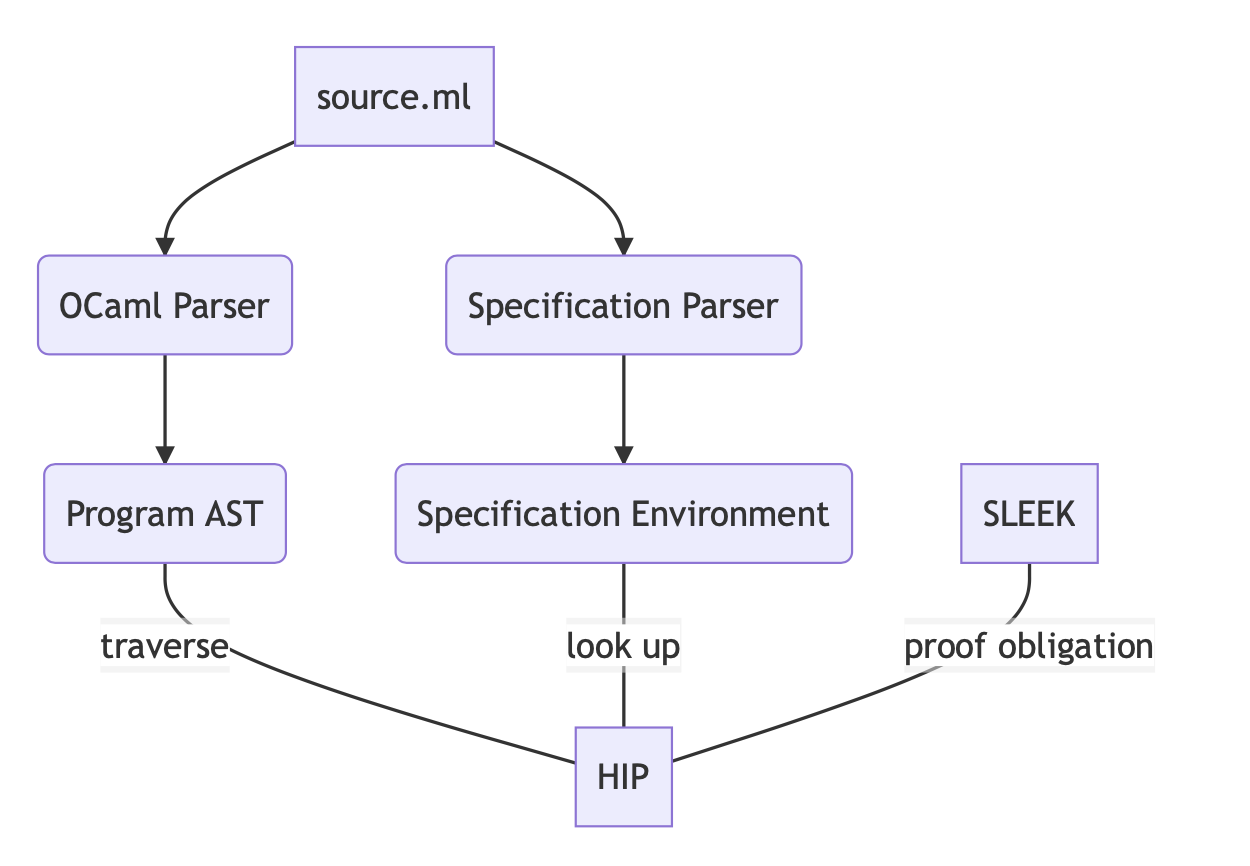
\includegraphics[width=0.8\linewidth]{report/pic/ch-Design/structure.png}
    \caption{Prototype system structure}
    \label{fig:structure}
\end{figure}

\subsection{Front-end Implementation}

We present the implementation of our front-end parser in this section. This section also serves as a guide to use our system. Our system takes an OCaml program \texttt{*.ml} as input. Users should program each method in the format of \texttt{let f x = ...} and only use the structures supported by our system. Otherwise the forward verifier will reject the input. The codes enclosed by \texttt{(*...*)} will be recognized as comments. However, if users write comments enclosed by \texttt{(*@ ...@*)}, they will be recognized by our specification parser and parsed into an abstract syntax tree for the forward verifier to use. Readers can refer to the next chapter to see several example programs that our system can accept and verify. Several implementation details are discussed below.

\paragraph{OCaml frontend} We make use of the OCaml 4.12.0 frontend library to parse the program part, so our forward verifier is based on the same program abstract syntax tree as the OCaml compiler accepts. The detail of the AST definition can be found in the OCaml compiler repository\footnote{https://github.com/ocaml/ocaml/blob/4.12/parsing/parsetree.mli}.

\paragraph{Specification parser} The OCaml parser library menhir is used in our implementation. The design of the specification abstract syntax tree follows the definition in \autoref{fig:AssASTcur}. To improve readability of the specification, users can write the top-level specification in the format of $\texttt{given} \ \vec{y} \texttt{ requires } \Phi_{\texttt{pre}} \texttt{ ensures[r] } \Phi_{\texttt{post}}$
The nested specifications in program assertions can be written as $\texttt{f(x)|=\{pre\}*->:r\{post\}}$. 




\section{Forward Verification}


\subsection{Logical reasoning rules}

We present a rule-based declaration for our forward verification system in \autoref{fig:choarelogic}. 
The judgement $\Sigma;\Gamma \provable \hoareabbr{\Delta_1}{e}{\texttt{r}}{\Delta_2}$ indicates \emph{if we evaluate $e$ in the initial state satisfying $\Delta_1$, then it terminates with a value, name it \texttt{r}, and a final state, which together satisfy $\Delta_2$}. All the rules are presented in a forward style, i.e. they expect precondition to be given before computing the postcondition. We write $\Delta[\mathtt{b/a}]$ to indicate the assertion obtained from replacing \texttt{a} by \texttt{b} in $\Delta$. We assume all the introduced anchors and variables are fresh.

\begin{figure}
\centering
\begin{mathpar}
    \inferrule[Fv-Method]{
        \mathcal{F} =  \textrm{Given } \vec{y}, \Phi_{\text{pre}} \rightarrowtail_{\mathtt{r} } \Phi_{\text{post}}
        \and
        \vec{x},\vec{y};P \provable\hoareabbr{ \Phi_{\text{pre}}}{e}{r}{ \Phi_{\text{post}}}
    } {
        \provable{\texttt{let f=}\lambda \vec{\mathtt{x}}.c \texttt{ where } \mathcal{F} }
    }[]\label{rule:fv-method}
    \\
    \inferrule[Fv-Spec]{
        \Sigma;\Gamma,\mathcal{F} \provable\hoareabbr{ \Delta_1}{e}{r}{ \Delta_2}
    } {
        \Sigma;\Gamma\provable\hoareabbr{\Delta_1\wedge\mathcal{F}}{e}{r}{\Delta_2}
    }[]\label{rule:fv-spec}
    \and
    \inferrule[Fv-Exists]{
        \Sigma,x;\Gamma \provable\hoareabbr{\Delta_1}{e}{r}{\Delta_2}
    } {
        \Sigma;\Gamma\provable\hoareabbr{\exists x.\Delta_1}{e}{r}{\Delta_2}
    }[]\label{rule:fv-exists}
    \\
    \inferrule[Fv-App-Par]{
            \Sigma;\Gamma \provable\hoareabbr{\Delta_0}{{f}}{\texttt{g}}{\Delta_1}
        \and
            \Sigma,\texttt{g};\Gamma \provable\hoareabbr{\Delta_1}{{x}}{\texttt{v}}{\Delta_2}
        \and
            \texttt{g}(\texttt{a},{\mathtt{\vec{b}}}) \ofspec 
                \mathcal{F} \in \Gamma
    } {
        \Sigma;\Gamma \provable\hoareabbr{\Delta_0}{f \ {x}}{h}{
            \Delta_2 \wedge
            \texttt{h}({\mathtt{\vec{b}}}) \ofspec \mathcal{F}[\mathtt{v/a}]
        }
    }[]\label{rule:fv-app-par}
    \\
        \inferrule[Fv-App-Full]{
            \Sigma;\Gamma \provable\hoareabbr{\Delta_0}{{f}}{\texttt{g}}{\Delta_1}
        \and
            \Sigma,\texttt{g};\Gamma \provable\hoareabbr{\Delta_1}{{x}}{\texttt{v}}{\Delta_2}
        \\
            \texttt{g}(\texttt{a}) \ofspec \textrm{Given } \vec{y},
                \Phi_{\text{pre}} \rightarrowtail_{\mathtt{r} } \Phi_{\text{post}} \in \Gamma \cup Spec(\Delta_2)
        \\
            \Delta_2 \entails             
                \Phi_{\text{pre}}(\vec{y})[\mathtt{v/a}]
        \and
            \Phi_{\text{post}}(\vec{y})[\mathtt{v/a,res/r}] \entails \Delta_3
    } {
        \Sigma;\Gamma \provable\hoareabbr{\Delta_0}{f \ {x}}{res}{
            \Delta_3
        }
    }[]\label{rule:fv-app-full}
    \\
    \inferrule[Fv-Match]{
         \Sigma;\Gamma \provable\hoareabbr{\Delta_1}{e}{v}{\Delta_2}
        \and
        \forall i,
             \Sigma, \mathtt{v}, \vec{\mathtt{x}_i} ;\Gamma \provable\hoareabbr{\Delta_2  \wedge
              \mathtt{v}::\texttt{cname}_i\left(\vec{\mathtt{x}_i}\right)}{e_i}{u}{\Delta_3}
    } {
        \Sigma; \Gamma \provable \hoareabbr{\Delta_1}{
            \texttt{match } e \texttt{ with } (\texttt{cname}_i \Rightarrow \lambda \vec{\mathtt{x}_i}.e_i)^*
        }{res}{\Delta_3[\mathtt{res/u}]}
    }[]\label{rule:fv-match}
    \and
    \inferrule[Fv-If]{
        \Sigma;\Gamma \provable\hoareabbr{\Delta_1}{e}{v}{\Delta_2}
        \and
        \Sigma,v;\Gamma \provable \hoareabbr{\Delta_2 \wedge \texttt{v} = \texttt{true}}{e_1}{u}{\Delta_3}
        \and \\
        \Sigma,v;\Gamma \provable \hoareabbr{\Delta_2 \wedge \texttt{v} = \texttt{false}}{e_2}{u}{\Delta_3}
    } {
        \Sigma; \Gamma \provable \hoareabbr{\Delta_1}{
            \texttt{if } e \texttt{ then } e_1 \texttt{ else } e_2 \ 
        }{res}{\Delta_3[\mathtt{res/u}]}
    }[]\label{rule:fv-if}
    \\
    \inferrule[Fv-Cst]{
    } {
        \Sigma; \Gamma \provable \hoareabbr{\Delta}{
          k
        }{res}{\Delta \wedge \texttt{res}=k }
    }[]\label{rule:fv-cst}
    \and
    \inferrule[Fv-Var]{
      \texttt{v} \in \Sigma
      \text{ or }
      \texttt{v}(\vec{x}) \ofspec \mathcal{F} \in \Gamma
    } {
        \Sigma; \Gamma \provable \hoareabbr{\Delta}{
          \texttt{v}
        }{res}{\Delta \wedge \texttt{res}= \texttt{v} }
    }[]\label{rule:fv-var}
    \\
    \inferrule[Fv-Fun-Eval]{
      \texttt{v}() \ofspec \textrm{Given } \vec{y}, \  \Phi_{\text{pre}} \rightarrowtail_{\mathtt{r} } \Phi_{\text{post}} \in \Gamma
      \and 
      \Delta \provable \Phi_{\text{pre}}(\vec{y})
    } {
        \Sigma; \Gamma \provable \hoareabbr{\Delta}{
          \texttt{v} \ 
        }{res}{\Delta \wedge \texttt{res}=v \wedge 
                \Phi_{\text{post}}(\vec{y})[\mathtt{res/r}] }
    }[]\label{rule:fv-fun-eval}
\end{mathpar}
    \caption{Proof rules of Hoare logic}
    \label{fig:choarelogic}
\end{figure}


We use $\Sigma$ to denote the dynamic context of logical variables and use $\Gamma$ to denote the context of specifications available for the expression to call. Our system keeps track of the context during forward verification for each method declaration. \nameref{rule:fv-spec} and \nameref{rule:fv-exists} allows the verifier to extract the method declarations or existential variables users write in the precondition to the context.


We use P to denote the program being checked. With pre/post conditions declared for each method in P, we can apply modular verification to a method’s body, as has been defined in \nameref{rule:fv-method}. When a new method is being verified, the variable context will be variables in the function arguments and \textsc{given} clause, and the specification context will be all the specifications in the program.

\nameref{rule:fv-app-par} deals with partial application, which basically creates a new instance of specification for a partially applied function. Note that the function and the argument should both be evaluated before creating the specification. \nameref{rule:fv-app-full} deals with full application. When all the arguments of the specification has been applied with program expressions, the verifier will check whether the precondition of the specification holds. Proving entailment will be presented in detail in the next section. If the entailment checker reports success, then the verifier can add the specified post condition to the inferred postcondition. Another thing to note is that the function specification may have variables or predicates to instantiate in the \textsc{given} clause, so the verifier should also infer the instances before proceeding the verification.

Apart from the standard structural rules such as \nameref{rule:fv-match}, \nameref{rule:fv-if}, \nameref{rule:fv-cst}, and \nameref{rule:fv-var}, our system also comprises a rule \nameref{rule:fv-fun-eval} for evaluating ``zero-ary'' function identifiers. Since our specification language supports nested function specifications in the assertion, the actual user-expected specification may be hidden in the assertion and needs unfolding. A verification example that uses this rule can be found in the next chapter.


\subsection{Implementation}

The logical rules above provide some general guidelines to verify a program annotated by user-provided specifications. To implement a forward verifier system, we should fix the order of applying these rules to make it more organized and easier to implement. Furthermore, the instantiating in \nameref{rule:fv-app-full} is in general an undecidable problem. Our verifier can only infer some predicate instances for a function application, and the inferred result may lead to a failure in proof. To address these issues, we list some key steps in implementing our forward verifier system.

The general structure of the forward verifier can be defined as a recursive function \texttt{infer\_exp} that takes as input the proof context $\mathcal{E}=(\Sigma,\Gamma)$, program expression $e$ and pre-condition $\Delta$. Due to the restriction we have discussed about instantiating, the output is designed in a non-deterministic style, i.e. the recursive function will output a set of possible solutions, each solution comprises the its proof context $\mathcal{E'}$, return value name $\mathtt{r}$, and inferred post-condition $\Delta'$.

To implement \texttt{infer\_exp}, we always normalize the input precondition using \nameref{rule:fv-spec} and \nameref{rule:fv-exists} on entry to extract the specifications into the proof context. Then the verifier will choose a rule based on the structure of the program expression. More than one possible inferred postcondition may be returned by \nameref{rule:fv-app-full}.

The recursion goes on following the syntax of the program expression $e$. After $e$ is evaluated, the verifier asks the entailment checker to check whether one of the triples $(\mathcal{E'}, \texttt{r}, \Delta')$ in the result can derive the expected post-condition. If so, the system can report that the method is verified w.r.t. the user-defined specification.


\section{Entailment checking}

At function call sites and the end of a method declaration, the forward verifier will generate proof obligations of assertion entailments. Our formulae are a combination of pure predicates and function specifications, where abstract predicates are involved. We take the satisfiability modulo theories (SMT) approach to discharge the proof obligations. In our project, we use Z3, an efficient SMT solver with specialized algorithms for solving background theories.


\begin{mathpar}
    \inferrule[Ent-Ass]{
        \Sigma \provable  \Delta_1
            \Rightarrow \Delta_2
        \and
        \Sigma; \Gamma; \Delta_1 \provable \vec{\mathcal{F}_1} \rhd \vec{\mathcal{F}_2} 
    } {
     \Delta_1 \wedge \vec{\mathcal{F}_1} \provable^{\Sigma;\Gamma}  \Delta_2 \wedge \vec{\mathcal{F}_2} 
    }[]\label{rule:ent-ass}
\end{mathpar}

Our job is to encode the proof entailments into a verification condition that Z3 accepts. Based on the solver result \texttt{SAT/UNSAT/UNKNOWN}, the entailment checker can return to the forward verifier whether the entailment succeeds. The general idea in \nameref{rule:ent-ass} is to verify both the derivation of the pure predicates and the \emph{subsumption} relation of the specifications. Note that the verification context is also used in the entailment checker, in that the variables that have been extracted into the context $\Sigma$ should be universally quantified, and that the specifications available in the context $\Gamma$ may also be used in the function subsumption check.

Since Z3 library has already provided a high-level API system for the OCaml programming language, most of the pure predicates such as arithmetic operations can be easily encoded as Z3 formulas. We will highlight several challenges and our solutions in the encoding.

\paragraph{Verifying with abstract predicates} The syntax of our specification language allows user to write logical expressions with abstract predicate ${f(\vec{e})}$.
What we mean by using an abstract predicate $f$ in a formula $\Delta_1(f) \entails \Delta_2(f)$ is that by replacing $f$ with any instance that matches the type signature of $f$ we can always prove $\Delta_1 \entails \Delta_2$. The abstract predicate $f$ is encoded as an uninterpreted function in the SMT formula. 

When there are uninterpreted formulas in the constraints, the Z3 solver will try to find instances of formulas that make the formula satisfiable. However, this solving process is different from our goal, since the \texttt{SAT} result for a direct encoding VC means $\exists f, \Delta_1(f) \entails \Delta_2(f)$ holds.
The trick here is to encode the negation of the formula, i.e. we add $\Delta_1 \wedge \neg \Delta_2$ to the constraints of the solver. The idea is that the negation of an existential quantifier is universal. Now if the solver returns \texttt{UNSAT}, the entailment checker should report success.


\paragraph{Verifying with concrete predicates} As the rule \nameref{rule:fv-app-full} shows, when we verify the application of a higher order specification with abstract predicates, we need to provide a concrete instance to predicates in the \textsc{given} clause. We will also see examples in the next chapter that users are able to write their own concrete predicates to help specify a function. To implement this feature, our solver will leave the original verification goal untouched, and add an extra constraint $\forall \vec{x}, f(\vec{x}) = \ldots $ to the Z3 constraints when certain predicates are instantiated.

\paragraph{Verifying function specifications} An important component of our assertions are function specifications. We use the notion of \emph{function subsumption}~\cite{Andrew2021Subsumption} to model our solution to the specification part. We say if $\mathcal{F}_1$ is a function subsumption of $\mathcal{F}_2$, that is $\mathcal{F}_1 <: \mathcal{F}_2$, then any function satisfying specification $\mathcal{F}_1$ can be used wherever a function satisfying $\mathcal{F}_2$ is required.

We look at the function part of \nameref{rule:ent-ass} in detail. We write $\Sigma; \Gamma; \Delta \provable \vec{\mathcal{F}_1} \rhd \vec{\mathcal{F}_2}$ to indicate that under variable context $\Sigma$ and specification context $\Gamma$, if pure proposition $\Delta$ holds, then all the function specification $\mathcal{F}$ required by $\vec{\mathcal{F}}_2$ can find a specification $\mathcal{G}$ in either $\vec{\mathcal{F}}_1$ or the specification context, which is of the same function name and is a subsumption of $\mathcal{F}$. This description is formally written in \nameref{rule:ent-fun-intro}.

\begin{mathpar}
    \inferrule[Ent-Fun-Intro]{
      \forall \mathcal{F} \in \vec{\mathcal{F}_2}, \quad
      \exists \mathcal{G} \in \vec{\mathcal{F}_1} \cup \Gamma, \mathcal{G} <:_{\Sigma, \Delta} \mathcal{F} 
    } {
      \Sigma; \Gamma; \Delta \provable \vec{\mathcal{F}_1} \rhd \vec{\mathcal{F}_2} 
    }[]\label{rule:ent-fun-intro}
    \and
    \inferrule[Fun-Sub]{
        \Sigma \entails \forall \vec{y}_2, \forall \vec{x}_2, \pi \wedge \Phi_2 \Rightarrow 
            \exists \vec{y}_1, \forall \vec{x}_1, \left( \Phi_1 \wedge \left(\forall \mathtt{r},  \Psi_1 \Rightarrow \Psi_2 \right) \right)
    } {
        \texttt{f}(\vec{x}) \ofspec \textrm{Given } \vec{y}_1,
                \Phi_{1} \rightarrowtail_{\mathtt{r} } \Psi_1
        <:_{\pi,\Sigma}
        \texttt{f}(\vec{x}) \ofspec \textrm{Given } \vec{y}_2,
                \Phi_{2} \rightarrowtail_{\mathtt{r} } \Psi_2 
    }[]\label{rule:fun-sub}
\end{mathpar}

To check whether a single function is a subsumption of the other, we encode the verification condition as \nameref{rule:fun-sub} shows. We assume that the function arguments and the return anchor name of the two functions have been renamed to be consistent. This encoding is in line with Kleymann’s adaptation-complete
rule of consequence~\cite{Kleymann1999HoareAux}. Note that the precondition is encoded in a \emph{contravariant} way since one can only strengthen the precondition of $\mathcal{F}_1$ to ensure its compatibility to  $\mathcal{F}_2$.



